\section{Resultados}
Para cada método utilizado para obter uma aproximação das raizes dos sistemas não lineares foi obtido 2 mapas, um deles (Gráficos do lado esquerdo) que representa se o método converge e para qual raiz ele convergiu, e o outro (Gráficos do lado direito) mostram a quantidade de iterações feitas até atingir o critério de parada de tolerância $ (\epsilon) =10^-6$ e iterações máxima ($k_{max}) = 20.$

Para esse exercício foi obtido os seguintes gráficos como resultado das convergências dos métodos de aproximação de sistemas não lineares:


\begin{figure}[tphb]
\centering
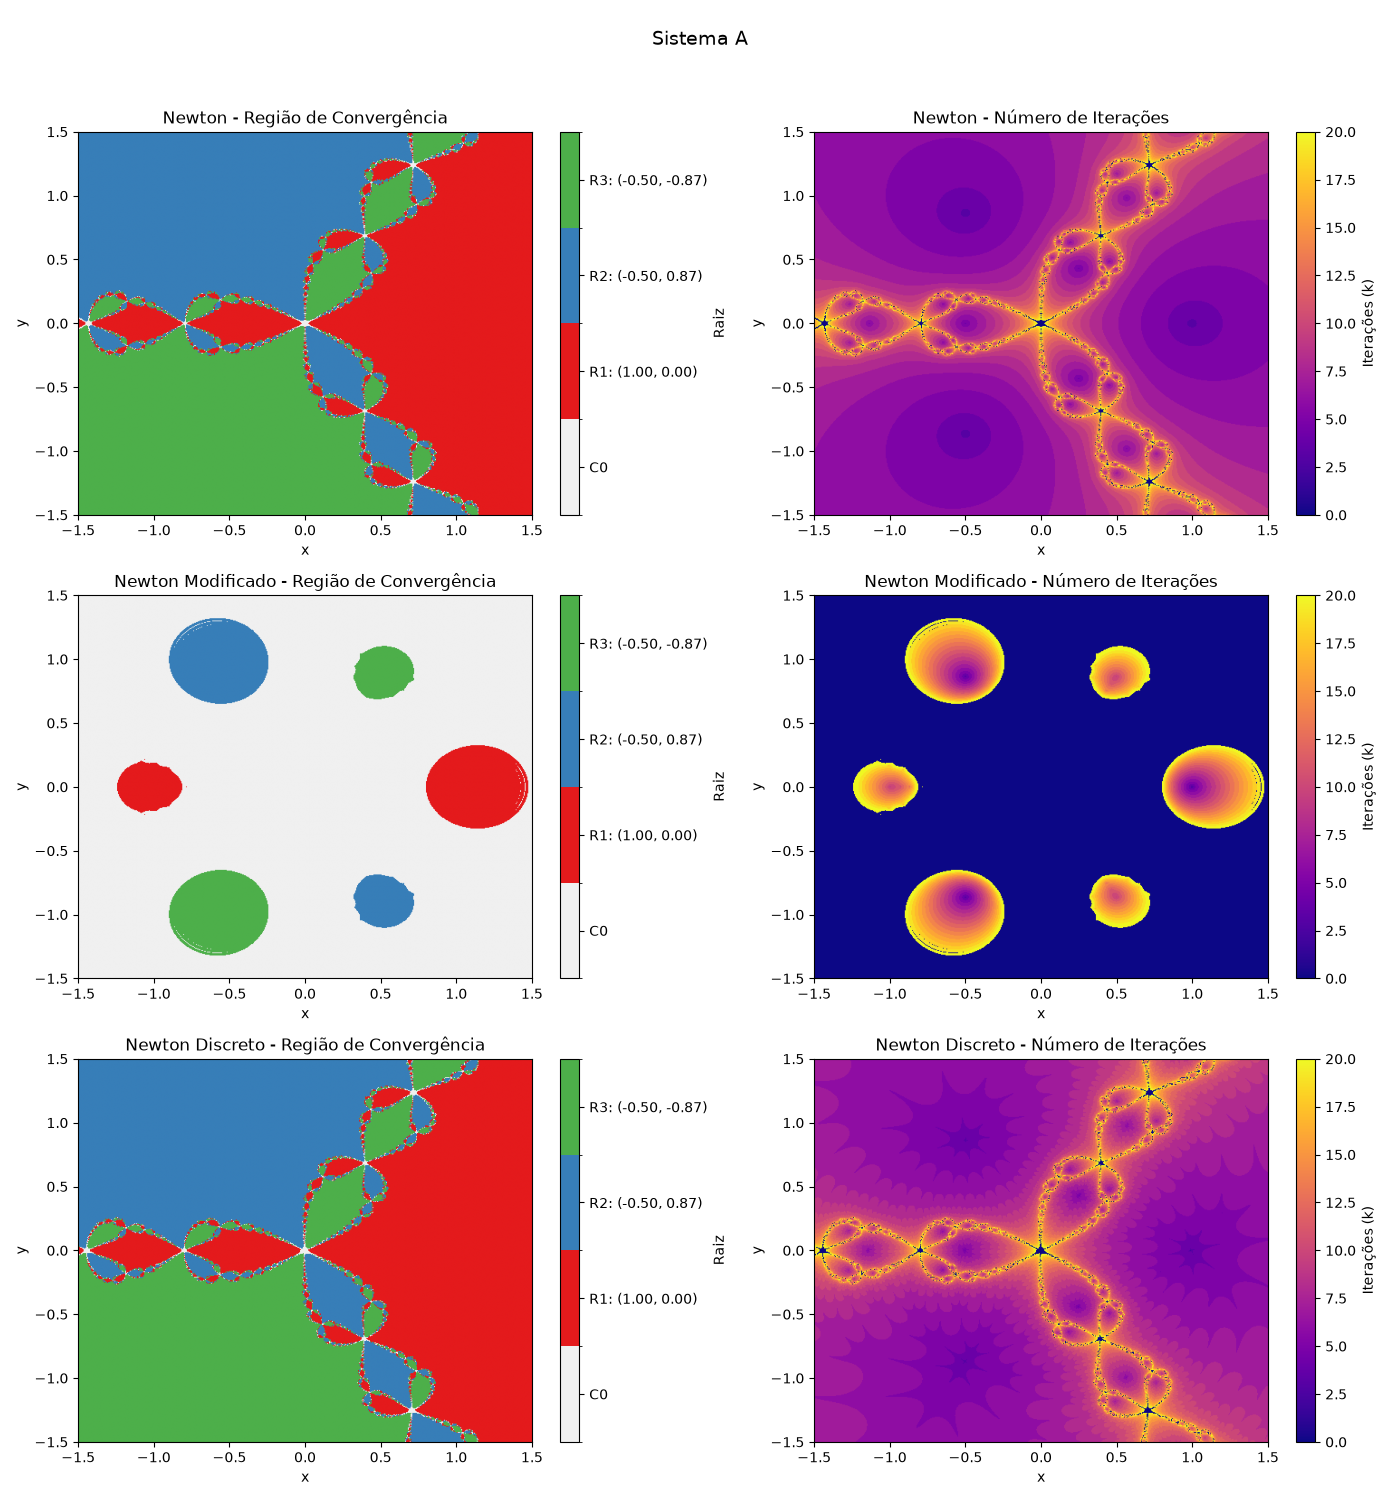
\includegraphics[width=0.6\textwidth]{sistemaA.png}
\caption{Gráficos das Convergências do Sistema $F_1(x,y)$}
\label{fig:rótulo}
\end{figure}

\begin{figure}[tphb]
\centering
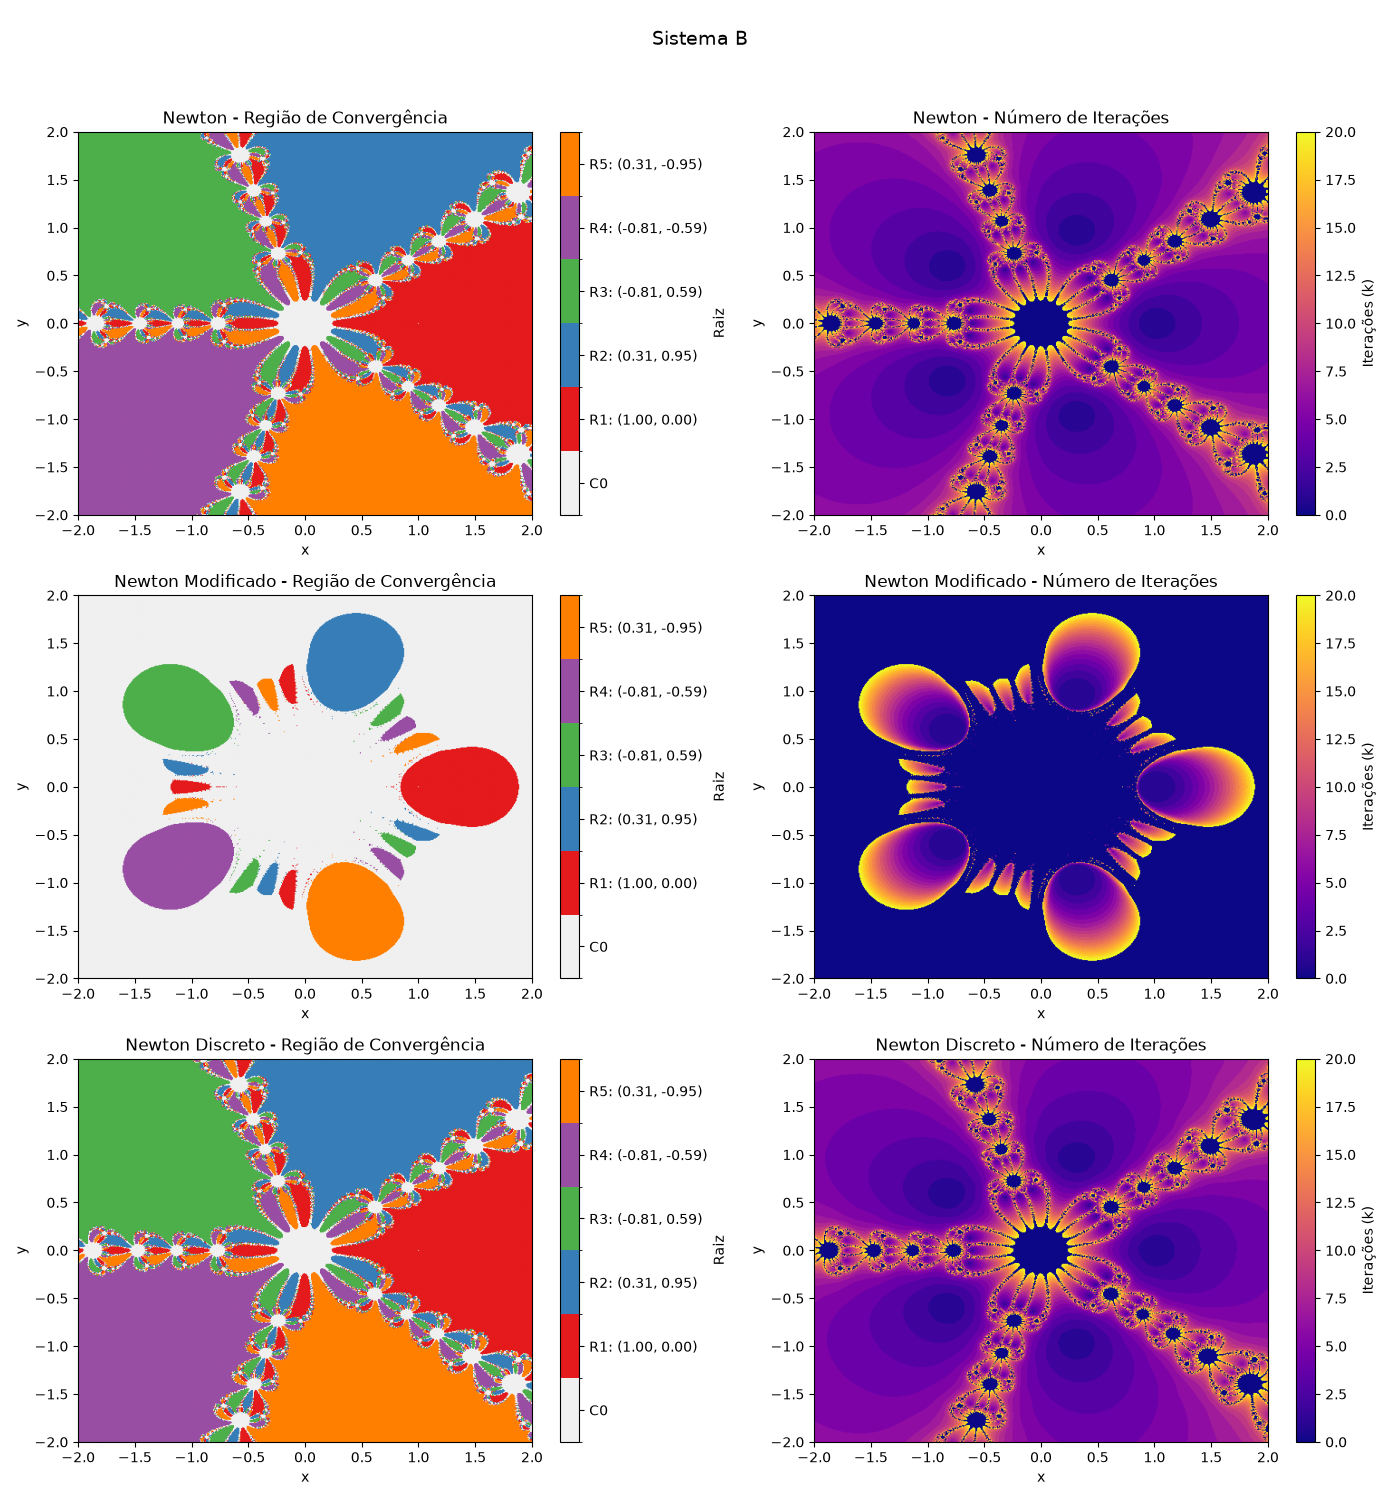
\includegraphics[width=0.6\textwidth]{sistemaB.png}
\caption{Gráficos das Convergências do Sistema $F_2(x,y)$}
\label{fig:rótulo}
\end{figure}